\documentclass[10pt,twocolumn,letterpaper]{article}

\usepackage{cvpr}
\usepackage{times}
\usepackage{epsfig}
\usepackage{graphicx}
\usepackage{amsmath}
\usepackage{amssymb}

% Include other packages here, before hyperref.

% If you comment hyperref and then uncomment it, you should delete
% egpaper.aux before re-running latex.  (Or just hit 'q' on the first latex
% run, let it finish, and you should be clear).
\usepackage[breaklinks=true,bookmarks=false]{hyperref}

\cvprfinalcopy % *** Uncomment this line for the final submission

\def\cvprPaperID{****} % *** Enter the CVPR Paper ID here
\def\httilde{\mbox{\tt\raisebox{-.5ex}{\symbol{126}}}}

% Pages are numbered in submission mode, and unnumbered in camera-ready
\ifcvprfinal\pagestyle{empty}\fi
%\setcounter{page}{4321}
\begin{document}

%%%%%%%%% TITLE
\title{Colorization}

\author{Vincent Billaut\\
Department of Statistics\\
Stanford University\\
{\tt\small vbillaut@stanford.edu}
% For a paper whose authors are all at the same institution,
% omit the following lines up until the closing ``}''.
% Additional authors and addresses can be added with ``\and'',
% just like the second author.
% To save space, use either the email address or home page, not both
\and
Matthieu de Rochemonteix\\
Department of Statistics\\
Stanford University\\
{\tt\small mderoche@stanford.edu}
\and
Marc Thibault\\
ICME\\
Stanford University\\
{\tt\small marcthib@stanford.edu}
}

\maketitle
%\thispagestyle{empty}

%%%%%%%%% ABSTRACT

% TODO for final report

%\begin{abstract}
%   The ABSTRACT is to be in fully-justified italicized text, at the top
%   of the left-hand column, below the author and affiliation
%   information. Use the word ``Abstract'' as the title, in 12-point
%   Times, boldface type, centered relative to the column, initially
%   capitalized. The abstract is to be in 10-point, single-spaced type.
%   Leave two blank lines after the Abstract, then begin the main text.
%   Look at previous CVPR abstracts to get a feel for style and length.
%\end{abstract}

%%%%%%%%% BODY TEXT
\section{Introduction}

The problem of colorization is one that comes quickly to mind when thinking about interesting challenges involving pictural data. Namely, the goal is to build a model that takes the greyscale version of an image (or even an actual "black and white" picture) and outputs its colorized version, as close to the original as possible (or at least realistic, if the original is not in colors).

One clear upside to this challenge is that any computer vision dataset, and even any image bank really, is a proper dataset for the colorization problem (the image itself is the model's expected output, and its greyscale version is the input to the model).

Classical approaches to this task, \eg \cite{cheng2015deep} and \cite{dahl2016tinyclouds}, aim at predicting an image as close as possible to the ground truth, and notably make use of a simple $L_2$ loss, which penalizes predictions that fall overall too far from the ground truth. As a consequence, the models trained following such methods usually tend to be very conservative, and to give desaturated, pale results.
On the contrary, authors of \cite{zhang2016colorful} take another angle and set their objective to be "\textit{plausible} colorization" (and not necessarily \textit{accurate}). One of their methods to validate their results was to set up a blind testing experiment where human subjects had to determine, between their prediction and the ground truth, which one seemed more realistic (and they achieved very good performance).

Our goal is to reproduce the approach of \cite{zhang2016colorful}, as we consider the implementation more challenging in the way the loss function and the prediction mechanism are designed, and the results more visually appealing.

If we reach satistfactory results in a timely manner, we will consider tackling the task of colorizing videos, which, in order to fully take advantage of the input format, will need to incorporate the notion of consistency between consecutive frames in a sequence.

\section{Problem statement}

\subsection{Datasets}

As previously stated, any dataset is proper for the colorization task, and we are currently working with subsets of both the SUN dataset \cite{xiao2010sun} and ImageNet \cite{russakovsky2015imagenet}.

More precisely, we are tackling a simplified version of our general task: correctly colorizing scenes that involve beaches and seashores. The idea behind this simplification is that restricting our model to rather consistent scenes, where we typically find the same patterns (the top of the scene is usually the sky, \ie blue, and the bottom usually sand, \ie yellow or brown, as shown by the example of Figure \ref{inex}), will enable us to have a working proof of concept, on top of which we can extend to bigger sets later.

\begin{figure}
\begin{center}
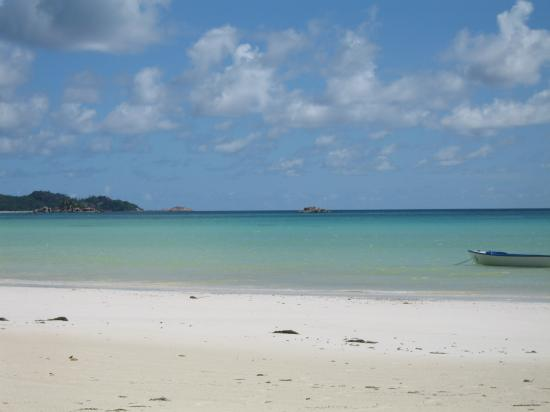
\includegraphics[width=200px]{img/beach.jpg}
\caption{Example of a picture from our reduced datasets (in this case, from ImageNet/beach)}
\label{inex}
\end{center}
\end{figure}

[WRITE HOW MANY PICTURES THIS REPRESENTS FOR EACH DATASET?]

\subsection{Expected results}

\subsection{Evaluation}

\section{Technical approach}

\section{Preliminary results}

\section{Next steps}

{\small
\bibliographystyle{ieee}
\bibliography{references}
}

\end{document}
